\section{Changes to the Bifurcation Structure}
\label{sec:add.change}

In this section, we will take a look at how changing the parameters as described in \Cref{sec:add.parameters} changes the bifurcation structure of the archetypal model.

\subsection{Numerical Overview of the Changes to the Bifurcation Structure}
\label{sec:add.change.num}

\Cref{fig:add.change.regions} shows diagrams depicting the borders of parameter regions with different symbolic sequences.
We will use these diagrams as basis for our exploration of the changes to the bifurcation structure.
The lower left corner of the diagrams is always in the period region with the stable cycle $\Cycle{\A^7\B^3\C^7\D^3}$.
The cycles in the upper left ($\Cycle{\A^6\B^3\C^6\D^3}$), upper right ($\Cycle{\A^6\B^4\C^6\D^4}$), lower right ($\Cycle{\A^7\B^4\C^7\D^4}$), and middle ($\Cycle{\A^7\B^3\C^6\D^4}$ and $\Cycle{\A^6\B^4\C^7\D^3}$) follow.

We introduce a short notation for the symbolic sequences here.
``Type A'' parameter regions where the cycle is associated with the symbolic sequence $\A^a\B^b\C^a\D^b$ are written as $P^{2 \cdot \left(a + b\right)}_b$
``Type B'' parameter regions where the coexisting twin cycles are associated with the symbolic sequences $\A^a\B^b\C^c\D^d$ and $\A^c\B^d\C^a\D^b$ where $c = a - 1$ and $d = b + 1$ are written as $P^{a + b + c + d}_b$.
So for example, the ``type A'' parameter region in the lower left corner of every diagram in \Cref{fig:add.change.regions} is written as $P^{20}_3$.

There is also a new type of parameter region that we call hybrid parameter regions with hybrid cycles.
Hybrid cycles are cycles that are asymmetrical like ``type B'' cycles and therefore also exist in pairs.
The difference to ``type B'' cycles is that for two hybrid twin cycles with the symbolic sequences $\A^a\B^b\C^c\D^d$ and $\A^c\B^d\C^a\D^b$ either $c \neq a - 1$ or $d \neq b + 1$.
The parameter region with such hybrid cycles is written as $\left[P^{2 \cdot \left(a + b\right)}_b \mid P^{2 \cdot \left(c + d\right)}_d\right]$ where $c \leq a$ and $d \geq b$.
This notation is chosen because of an operation that is introduced in the later \Cref{sec:add.add.halved}.

The four different diagrams in \Cref{fig:add.change.regions} show the evolution at different points during the transition from \Cref{fig:add.arch} to \Cref{fig:add.arch.new}.
For this, the parameter values for $a_L$ and $b_L$ are chosen along a line given by \Cref{equ:add.change.paramline}.
\begin{align}
	a_L = \frac{5}{2} - 3 \cdot b_L
	\label{equ:add.change.paramline}
\end{align}

\begin{figure}
	\centering
	\subfloat[$a_L = 3.5, b_L = -0.\overline{3}$]{
		\includegraphics[width=.5 \textwidth]{62_MinimalRepr_Adding/2D_Regions_3.5/Manual/result.png}
		\label{fig:add.change.regions.1}
	}
	\subfloat[$a_L = 2.8, b_L = -0.1$]{
		\includegraphics[width=.5 \textwidth]{62_MinimalRepr_Adding/2D_Regions_2.8/Manual/result.png}
		\label{fig:add.change.regions.2}
	} \\
	\subfloat[$a_L = 2.725, b_L = -0.075$]{
		\includegraphics[width=.5 \textwidth]{62_MinimalRepr_Adding/2D_Regions_2.725/Manual/result.png}
		\label{fig:add.change.regions.3}
	}
	\subfloat[$a_L = 2.5, b_L = 0$]{
		\includegraphics[width=.5 \textwidth]{62_MinimalRepr_Adding/2D_Regions_2.5/Manual/result.png}
		\label{fig:add.change.regions.4}
	}
	\caption[Changes to the bifurcation structures of the archetypal model during its transition to the increasing archetypal model]{
		2D boundary scans of the archetypal model showing the borders of parameter regions that are associated with different symbolic sequences.
		The parameter $g_R\left(\frac{1}{2}\right) = \frac{1}{2} + \frac{1}{40}$ is fixed in every diagram.
		The parameters $a_L$ and $b_L$ are fixed, but different in every diagram.
		Their values are on the line given by \Cref{equ:add.change.paramline}.
		The parameters $\alpha = g_R\left(\frac{1}{4}\right)$ and $\beta = c_L$ are varied.
		The diagrams illustrate the changes to the bifurcation structure in the archetypal model when transitioning to the increasing archetypal model.
	}
	\label{fig:add.change.regions}
\end{figure}

First, we will examine the disappearance of the ``type B'' parameter regions.
After that, we will examine the appearance of period-adding structures between the chains of the same period.

\subsection{Disappearance of ``Type B'' Parameter Regions}
\label{sec.change.disb}

For \Cref{fig:add.change.regions.1,fig:add.change.regions.2}, the ``type B'' parameter region $Q^{20}_3$ is complete.
In \Cref{fig:add.change.regions.4}, it is gone completely, instead the two ``type A'' parameter regions $P^{20}_3$ and $P^{20}_4$ now overlap.
\todo{In regions figure 3: labels $P^{20}_2$ wrong, should be $P^{20}_4$}

In between those two stages, we can see how the ``type B'' parameter region $Q^{20}_3$ disappears.
\Cref{fig:add.change.regions.3} shows the ``type A'' parameter regions $P^{20}_3$ and $P^{20}_4$ overlapping.
The point, where their boundaries cross is in the middle of where the ``type B'' parameter region was in \Cref{fig:add.change.regions.2}.
This point is also where the ``type B'' parameter region now ends.

\todo{Labels in figure wrong!}
\todo{In cobweb diagrams: enhance cycles at borders}
\begin{figure}
	\centering
	\subfloat[Regions]{
		\includegraphics[width=.3 \textwidth]{62_MinimalRepr_Adding/2D_Regions_2.675/Manual/result.png}
		\label{fig:add.change.disb.regions}
	}
	\subfloat[Cobweb at point $A$]{
		\includegraphics[width=.3 \textwidth]{62_MinimalRepr_Adding/Cob_2.675_A/Manual/result.png}
		\label{fig:add.change.disb.cob.A}
	}
	\subfloat[Cobweb at point $B$]{
		\includegraphics[width=.3 \textwidth]{62_MinimalRepr_Adding/Cob_2.675_B/Manual/result.png}
		\label{fig:add.change.disb.cob.B}
	}
	\caption{Disappearance of the ``type B'' parameter region}
\end{figure}

\Cref{fig:add.change.disb.regions} shows the same thing as \Cref{fig:add.change.regions.3} again but at parameter value closer to the diappearence of the ``type B'' parameter region.
We can see that the point where the boundaries of the ``type A'' parameter regions cross moved right and the ``type B'' parameter region got smaller.
This point is called a codimension-2 point because at this point, two bifurcations happen at the same time to the same cycle.

We know from \Cref{sec:arch.bif.sum} that the \gls{bcb} at the upper boundary of the ``type A'' parameter region $P^{20}_3$ is $\BCB_{d_1, d_3}^{\underline{\A}^7\B^3\underline{\C}^7\D^3}$.
And the \gls{bcb} at the lower boundary of the ``type A'' parameter region $P^{20}_4$ is $\BCB_{d_1, d_3}^{\A^6\underline{\B}^4\C^6\underline{\D}^4}$.
At the codimension-2 point, both these \glspl{bcb} happen at the same time and both cycles vanish.
We can see in \Cref{fig:add.change.disb.cob.A} that the ``type A'' cycles are very close to the borders $d_1$ and $d_3$, respectively.

We also know that the \glspl{bcb} at the top of the ``type B'' parameter region $Q^{20}_3$ are $\BCB_{d_1}^{\underline{\A}^7\B^3\C^6\D^4}$ and $\BCB_{d_3}^{\A^6\B^4\underline{\C}^7\D^3}$.
And the \glspl{bcb} at the lower boundary are $\BCB_{d_3}^{\A^7\B^3\C^6\underline{\D}^4}$ and $\BCB_{d_1}^{\A^7\underline{\B}^3\C^6\D^4}$.
At the codimension-2 point, both \glspl{bcb} $\BCB_{d_1}^{\underline{\A}^7\B^3\C^6\D^4}$ and $\BCB_{d_3}^{\A^7\B^3\C^6\underline{\D}^4}$ happen to the cycle $\Cycle{\A^7\B^3\C^6\D^4}$ at the same time and it vanishes.
Because of the symmetry, the \glspl{bcb} $\BCB_{d_3}^{\A^6\B^4\underline{\C}^7\D^3}$ and $\BCB_{d_1}^{\A^7\underline{\B}^3\C^6\D^4}$ happen to the cycle $\Cycle{\A^6\B^4\C^7\D^3}$ at the same time and it vanishes also.

This codimension-2 point moves right with higher values for $b_L$ along our line.
As soon as the codimension-2 point crosses the right boundary of the ``type B'' parameter region, the ``type B'' parameter region ceases to exist.
Instead, now the two ``type A'' parameter regions overlap without the codimension-2 point.
This new overlapping regions is bounded by simple ``type A'' boundary \glspl{bcb} as they are discussed in \Cref{sec:arch.bif.sum}.

\todo{Confirm bcbs with cobweb diagrams}

\todo{Order of left most cycle and other cycle => type B or type A. idk}

\subsection{Appearance of Period-adding structures}

In this section we will explore the appearance of the period-adding structures in between the chains of the same period.
This happens at the horizontal boundaries between ``type A'' parameter regions of different chains, as well as at the vertical boundaries.
We will first take care of the horizontal period-adding structures and then move on to the vertical period-adding structures.

\subsubsection{Horizontal Period-adding Structures}

In \Cref{fig:add.change.regions.1}, the ``type A'' parameter regions $P^{20}_3$ and $P^{18}_3$, as well as $P_{22}_4$ and $P^{20}_4$ overlap.
This changes in \Cref{fig:add.change.regions.2}.
Here only the ``type A'' parameter regions $P^{20}_3$ and $P^{18}_3$ overlap, the parameter regions $P_{22}_4$ and $P^{20}_4$ stopped overlapping.
Instead, in the space between the two ``type A'' parameter region there are now two asymmetric coexisting twin cycles $\Cycle{\A^8\B^3\C^8\D^2}$ and $\Cycle{\A^8\B^2\C^8\D^3}$.
Those cycles are \textbf{not} ``type B'' cycles, because they only differ in the number of points on the branches $f_\B$ and $f_\D$.
Instead, we will call them hybrid cycles and ``type B'' cycles are a special case of hybrid cycles.
The notation $\left[P^{22}_4 \mid P^{20}_4\right]$ used in the diagrams was introduced in \Cref{sec:add.change} and is formally defined later in \Cref{sec:add.add.halved}.
Later in \Cref{fig:add.change.regions.4}, the ``type A'' parameter regions $P^{20}_3$ and $P^{18}_3$ also stop overlapping.
In between, there are also hybrid cycles, $\Cycle{\A^7\B^3\C^6\D^3}$ and $\Cycle{\A^6\B^3\C^7\D^3}$.
This parameter region is therefore labeled $\left[P^{20}_3 \mid P^{18}_3\right]$.

In between \Cref{fig:add.change.regions.2,fig:add.change.regions.3}, the ``type A'' parameter regions $P_{22}_4$ and $P^{20}_4$ don't stop overlapping completely.
Instead, they only stop overlapping on the left side of their shared boundaries and the rest is not pictured in these diagrams.
\Cref{fig:add.change.appa.hor.regions} shows better what happens to this overlapping region between \Cref{fig:add.change.regions.1,fig:add.change.regions.4}.
We also have a codimension-2 point that moves right as was the case in \Cref{sec:add.change.disb}.

\todo{Regions: labels wrong}
\todo{Cobwebs: enhance borders, replace (c), wrong pic}
\begin{figure}
	\centering
	\subfloat[Regions]{
		\includegraphics[width=.3 \textwidth]{62_MinimalRepr_Adding/2D_Regions_2.8_add_hor/Manual/result.png}
		\label{fig:add.change.appa.hor.regions}
	}
	\subfloat[At point $A$]{
		\includegraphics[width=.3 \textwidth]{62_MinimalRepr_Adding/Cob_2.8_add_hor_A/Manual/result.png}
		\label{fig:add.change.appa.hor.cob.A}
	}
	\subfloat[At point $B$]{
		\includegraphics[width=.3 \textwidth]{62_MinimalRepr_Adding/Cob_2.8_add_hor_A/Manual/result.png}
		\label{fig:add.change.appa.hor.cob.B}
	}
	\caption{Appearance of the horizontal period-adding cascade}
\end{figure}

We know from \Cref{sec:arch.bif.sum} that the \gls{bcb} at the upper boundary of the ``type A'' parameter region $P^{22}_4$ is $\BCB_{d_1, d_3}^{\underline{\A}^7\B^4\underline{\C}^7\D^4}$.
And the \gls{bcb} at the lower boundary of the ``type A'' parameter region $P^{20}_4$ is $\BCB_{d_1, d_3}^{\A^6\underline{\B}^4\C^6\underline{\D}^4}$.
Both these \glspl{bcb} are at the upper and lower boundaries of the overlapping region $P^{22}_4 \Cup P^{20}_4$.
At the codimension-2 point, both these \glspl{bcb} happen at the same time and both cycles vanish.
We can see in \Cref{fig:add.change.appa.hor.cob.A} that the ``type A'' cycles are very close to the borders $d_1$ and $d_3$, respectively.

This codimension-2 point moves right with higher values for $b_L$ along our line.
As soon as the codimension-2 point crosses the right boundary of either the ``type A'' parameter region $P^{22}_4$ or $P^{20}_4$, the overlapping parameter region $P^{22}_4 \Cup P^{20}_4$ ceases to exist.
Instead, there is space between the two ``type A'' parameter regions where the are now two hybrid cycles and period-adding between the hybrid cycles and either ``type A'' parameter region.

\todo{Labels for bifurcations missing underline}
\begin{figure}
	\centering
	\includegraphics[width=.7 \textwidth]{62_MinimalRepr_Adding/1D_Bif_2.8_add_hor_AU/Manual/result.png}
	\caption{Bifurcation diagram at the upper boundary of $\left[P^{22}_4 \mid P^{20}_4\right]$}
	\label{fig:add.change.appa.hor.bif}
\end{figure}

We assume that the \glspl{bcb} bounding the parameter regions with hybrid cycles follow the same rules as the \glspl{bcb} bounding the ``type B'' parameter regions.
\Cref{fig:add.change.appa.hor.bif} confirms this for the upper boundary.
So it is bounded at the top by the \glspl{bcb} $\BCB_{d_1}^{\underline{\A}^7\B^4\C^6\D^4}$ and $\BCB_{d_3}^{\A^6\B^4\underline{\C}^7\D^4}$.
And bounded at the bottom by the \glspl{bcb} $\BCB_{d_3}^{\A^7\B^4\C^6\underline{\D}^4}$ and $\BCB_{d_1}^{\underline{\A}^6\B^4\C^7\D^4}$.
At the codimension-2 point, both \glspl{bcb} $\BCB_{d_1}^{\underline{\A}^7\B^4\C^6\D^4}$ and $\BCB_{d_3}^{\A^7\B^4\C^6\underline{\D}^4}$ happen to the cycle $\Cycle{\A^7\B^4\C^6\D^4}$ at the same time and it vanishes.
Because of the symmetry, the \glspl{bcb} $\BCB_{d_3}^{\A^6\B^4\underline{\C}^7\D^4}$ and $\BCB_{d_1}^{\A^6\underline{\B}^4\C^7\D^4}$ happen to the cycle $\Cycle{\A^6\B^4\C^7\D^4}$ at the same time and it vanishes also.

\todo{also confirmed by cobweb with enhanced cycles at borders}

\todo{Parallels to disappearing type B}

\todo{old:}

In \Cref{sec:minrep.adding.disapp.typeB}, we noted that the asymmetry of the ``type B'' cycles is caused by the negative slope of the function at the left border of branches $f_\A$ and $f_\C$.
Since this maps the cycle that starts further left to the right side of the other cycle.
\todo{
	explain better: diff number of points on branches B and D each (type B) therefore reordering necessary for asymm.
	type b also: split at $d_1, d_3$ as well as $d_2$ and $d_0$, here only $d_1, d_3$ (two boundaries).
	here same number of points so there must be no reordering for asymm
}
This is not the case for the cycles at this point, both cycles start at a point on the branch $f_\A$ with a positive slope and therefore keep the same order.
\todo{positive slope important for period adding!}

\subsubsection{Vertical}

\todo{Regions: labels wrong}
\todo{Cobwebs: replace (c) and enhance cycles at borders}
\begin{figure}
	\centering
	\subfloat[Regions scan before period-adding\\at $a_L = 2.8, b_L = -0.1$]{
		\includegraphics[width=.4 \textwidth]{62_MinimalRepr_Adding/2D_Regions_2.8_add_vert/Manual/result.png}
		\label{fig:minrep.add.app.vert.reg.before}
	}
	\subfloat[Regions with period-adding\\at $a_L = 2.65, b_L = -0.05$]{
		\includegraphics[width=.4 \textwidth]{62_MinimalRepr_Adding/2D_Regions_2.65_add_vert/Manual/result.png}
		\label{fig:minrep.add.app.vert.reg.with}
	} \\
	\subfloat[At point $A$]{
		\includegraphics[width=.4 \textwidth]{62_MinimalRepr_Adding/Cob_2.8_add_vert_A/Manual/result.png}
		\label{fig:minrep.add.app.vert.cob.A}
	}
	\subfloat[At point $B$]{
		\includegraphics[width=.4 \textwidth]{62_MinimalRepr_Adding/Cob_2.65_add_vert_B/Manual/result.png}
		\label{fig:minrep.add.app.vert.cob.B}
	}
	\caption{Appearance of the vertical period-adding cascade}
	\label{fig:minrep.add.app.vert}
\end{figure}

For the vertical period-adding cascade, it is similar.
This time one parameter region scan is not enough because the boundaries of $P_{10}^3$ and $P_{11}^4$ are parallel and therefor $P_{10}^3 \bigcup P_{11}^4$ and $P_{10}^3 \oplus P_{11}^4$ can't exist at the same parameter values of $a_L$ and $b_L$.
\Cref{fig:minrep.add.app.vert.reg.before} shows the situation before the vertical period-adding cascade appears.
Here we can see the overlap of the two ``type A'' parameter regions $P_{10}^3$ and $P_{11}^4$.
When changing the parameters a little, we get \Cref{fig:minrep.add.app.vert.reg.with}.
Here the two ``type A'' parameter regions drifted apart and in between them, there is the parameter region $P_{10}^3 \oplus P_{11}^4$.
The notation hints at the period-adding-like nature of this parameter region.

As with the horizontal period-adding cascade, the cycles here are asymmetrical, but not of ``type B''.
\Cref{fig:minrep.add.app.vert.cob.B} shows the cycles at point $B$, in the period adding cascade, $\Cycle{\A^7\B^3\C^7\D^4}$ and its twin $\Cycle{\A^7\B^4\C^7\D^3}$.
Again, interpreted in the context of the halved model, these cycles are both $\Cycle{\L^7\R^3\L^7\R^4} \equiv \Cycle{\L^7\R^4\L^7\R^3}$.
But this time, the splits are not at borders $d_1$ and $d_3$, but at $d_0$ and $d_2$.
\todo{odd number of splits => no neg slope needed for asymmetry. odd number => needed (reorders cycles)}

\begin{figure}
	\centering
	\includegraphics[width=.7 \textwidth]{62_MinimalRepr_Adding/1D_Bif_2.65_add_vert_BR/Manual/result.png}
	\caption{Bifurcation diagram of the right boundary of $P_{10}^3 \oplus P_{11}^4$}
	\label{fig:minrep.add.app.vert.bif.BR}
\end{figure}

Here, the period-adding region opened up enough to see the next stage, colored in purple.
As with the previous bifurcations of the first stage of the horizontal period-adding cascade, the bifurcations are similar to the bifurcations of ``type B'' cycles in \Cref{sec:minrep.bif.R}.
They involve the borders $d_0$ and $d_2$.
\todo{etc}

\subsection{Summary of the Changes to the Bifurcation Structure}

This section summarizes all the changes that happen to the \gls{pi} structure of the archetypal model when the parameters are changed in such a way that \gls{pal} structures emerge.
Furthermore, it provides an explanation for why the \gls{pi} structure of the archetypal model is impossible with only increasing branches.

\subsubsection{Schematics and Summary of the Changes}

\begin{figure}
	\centering
	\subfloat[]{
		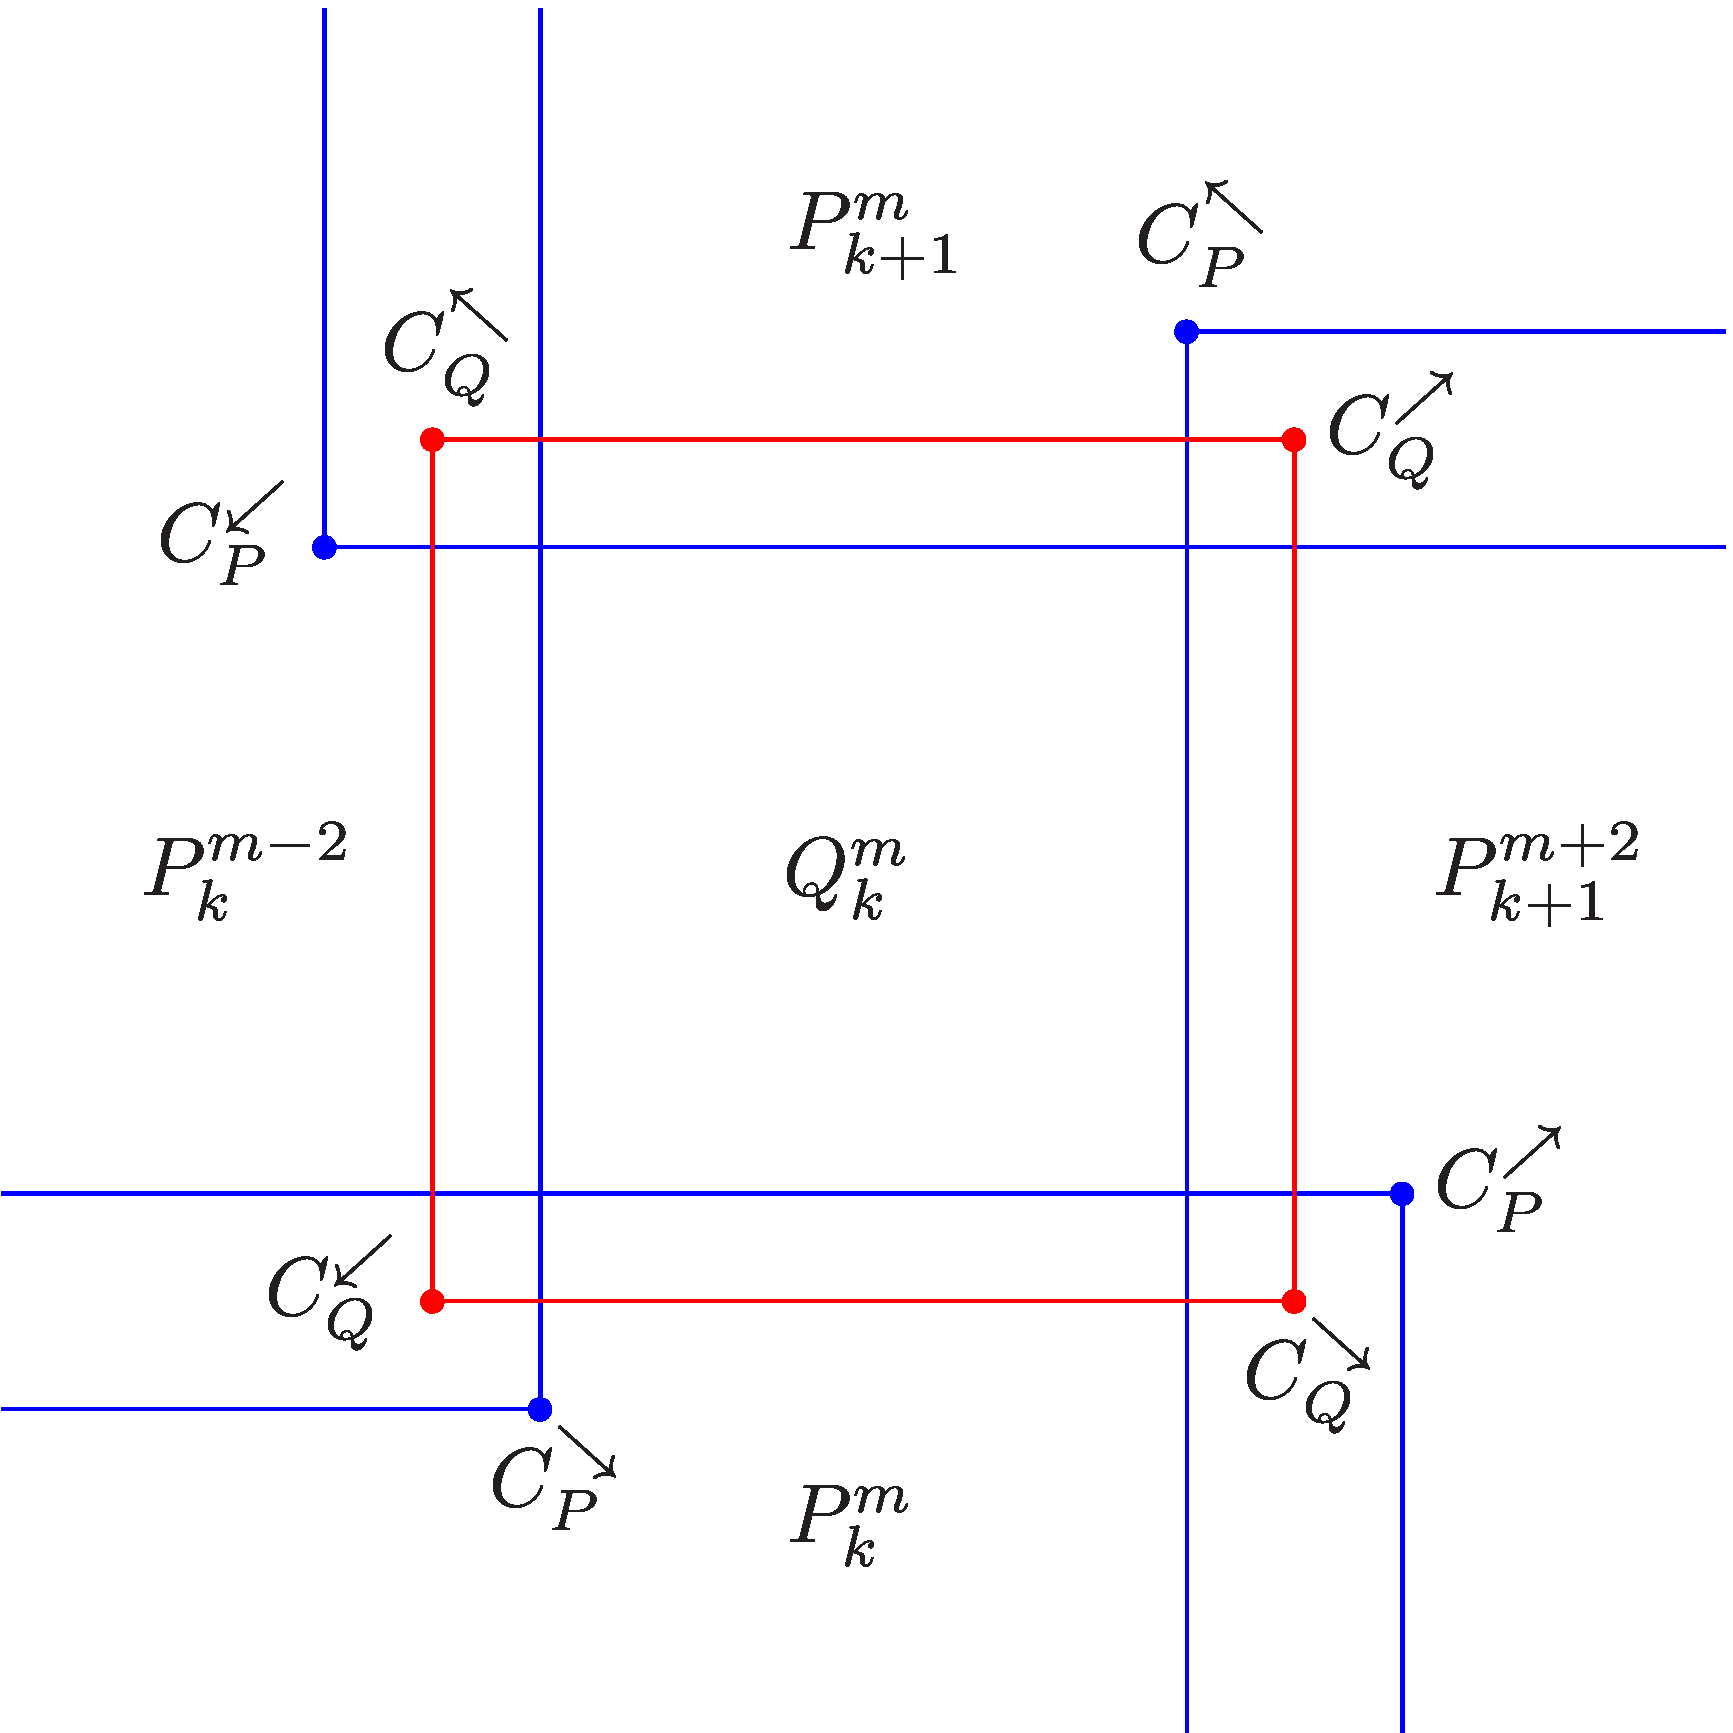
\includegraphics[width=.4 \textwidth]{../Figures/7/7.9a/result.png}
		\label{fig:add.change.schema.a}
	}
	\subfloat[]{
		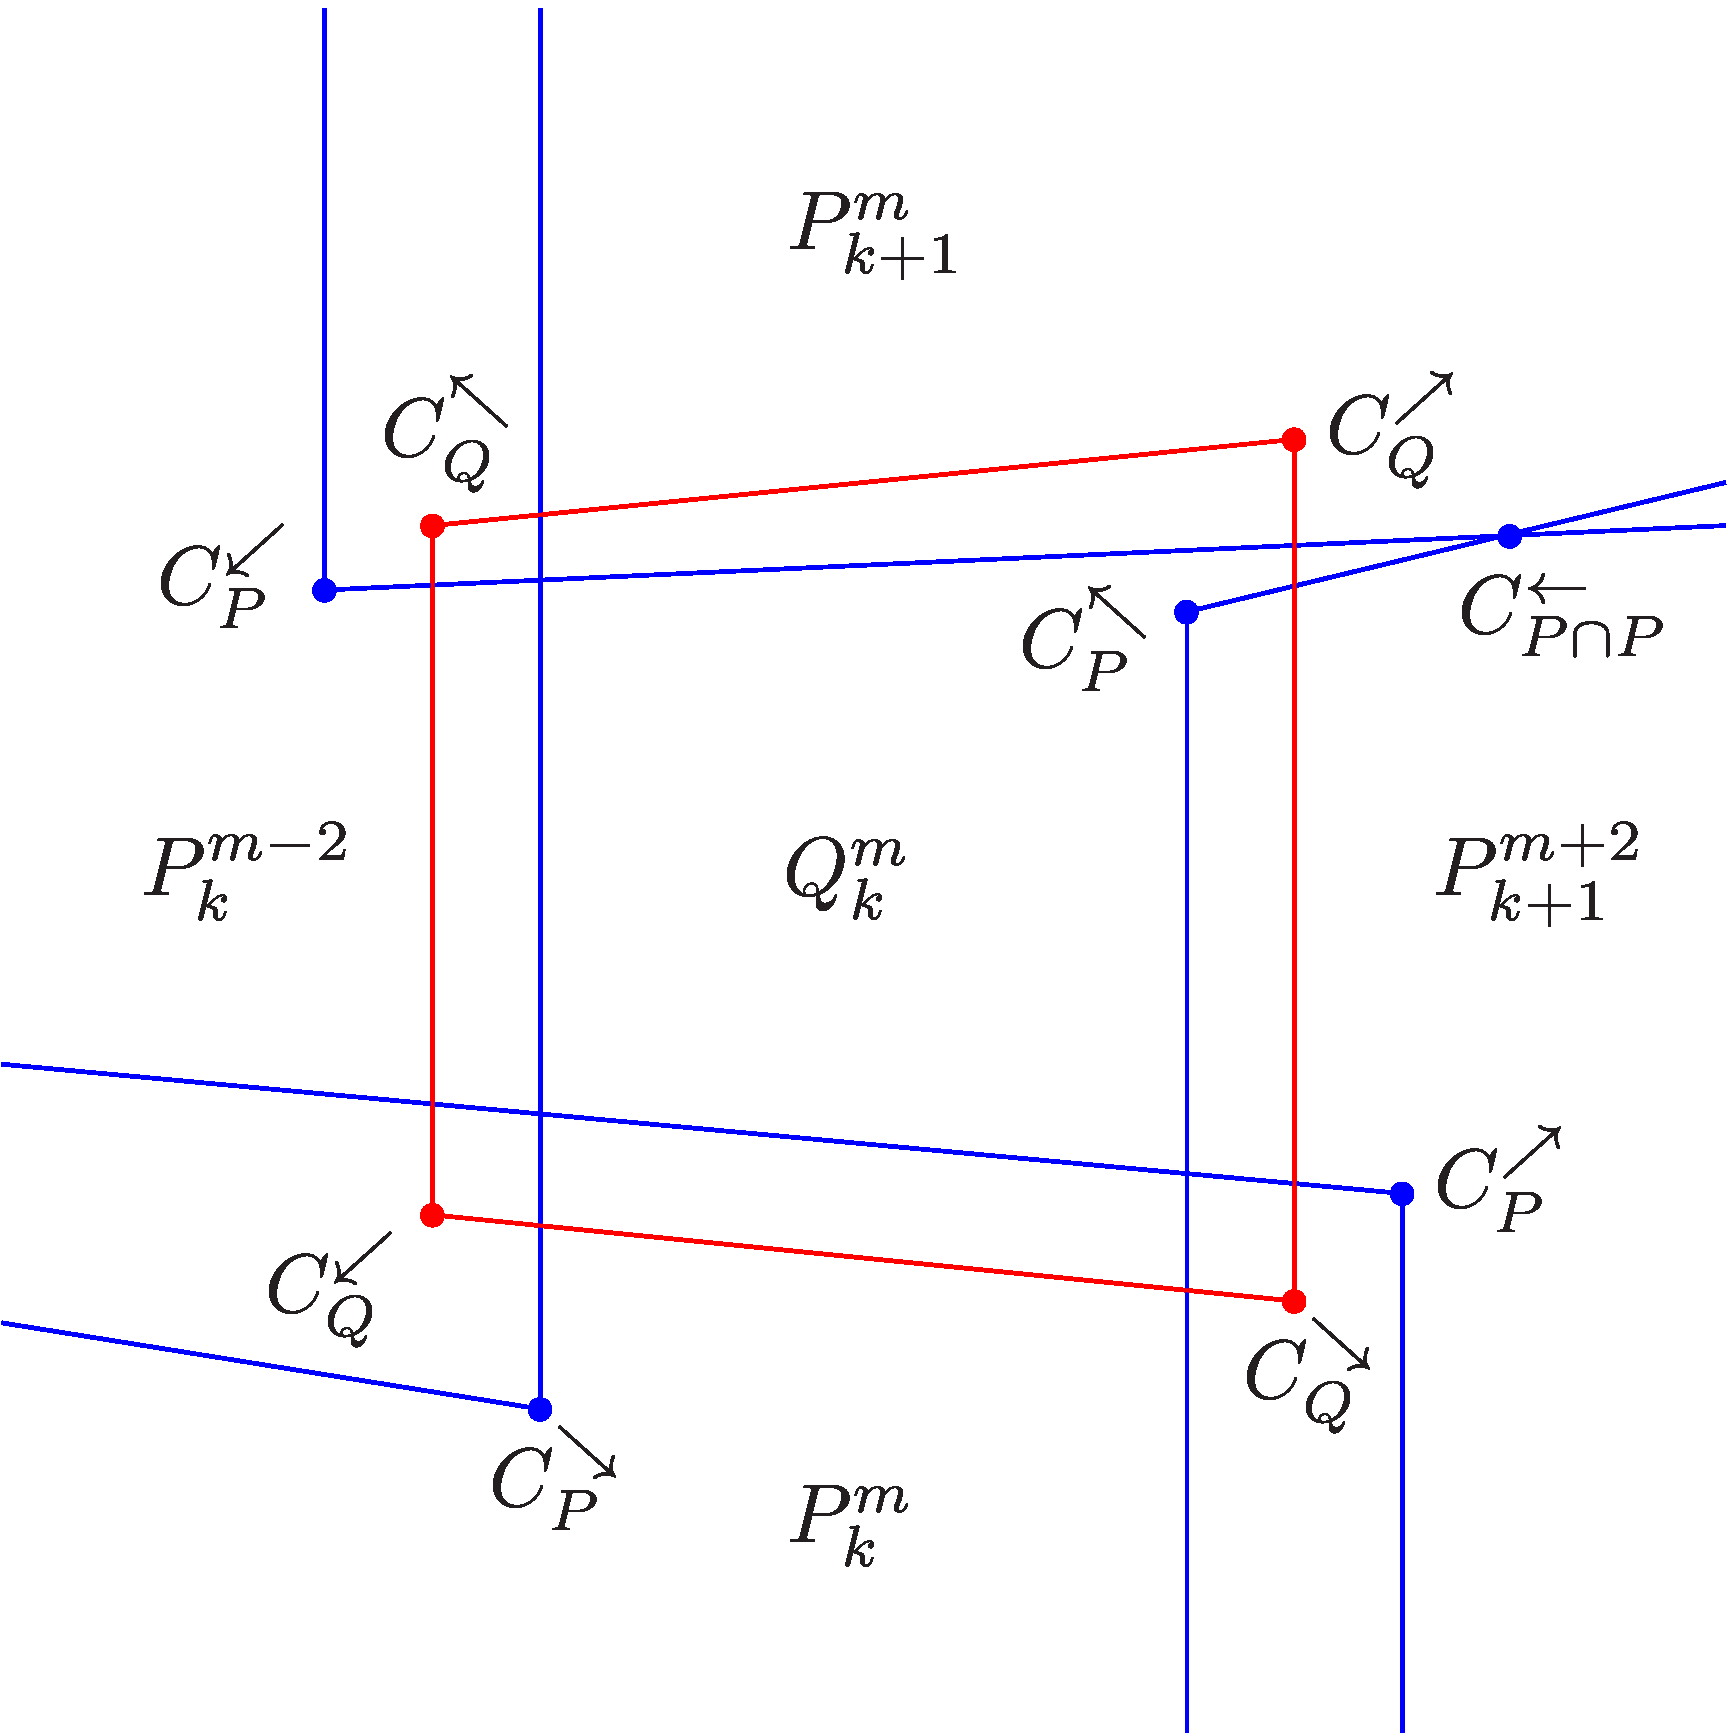
\includegraphics[width=.4 \textwidth]{../Figures/7/7.9b/result.png}
		\label{fig:add.change.schema.b}
	} \\
	\subfloat[]{
		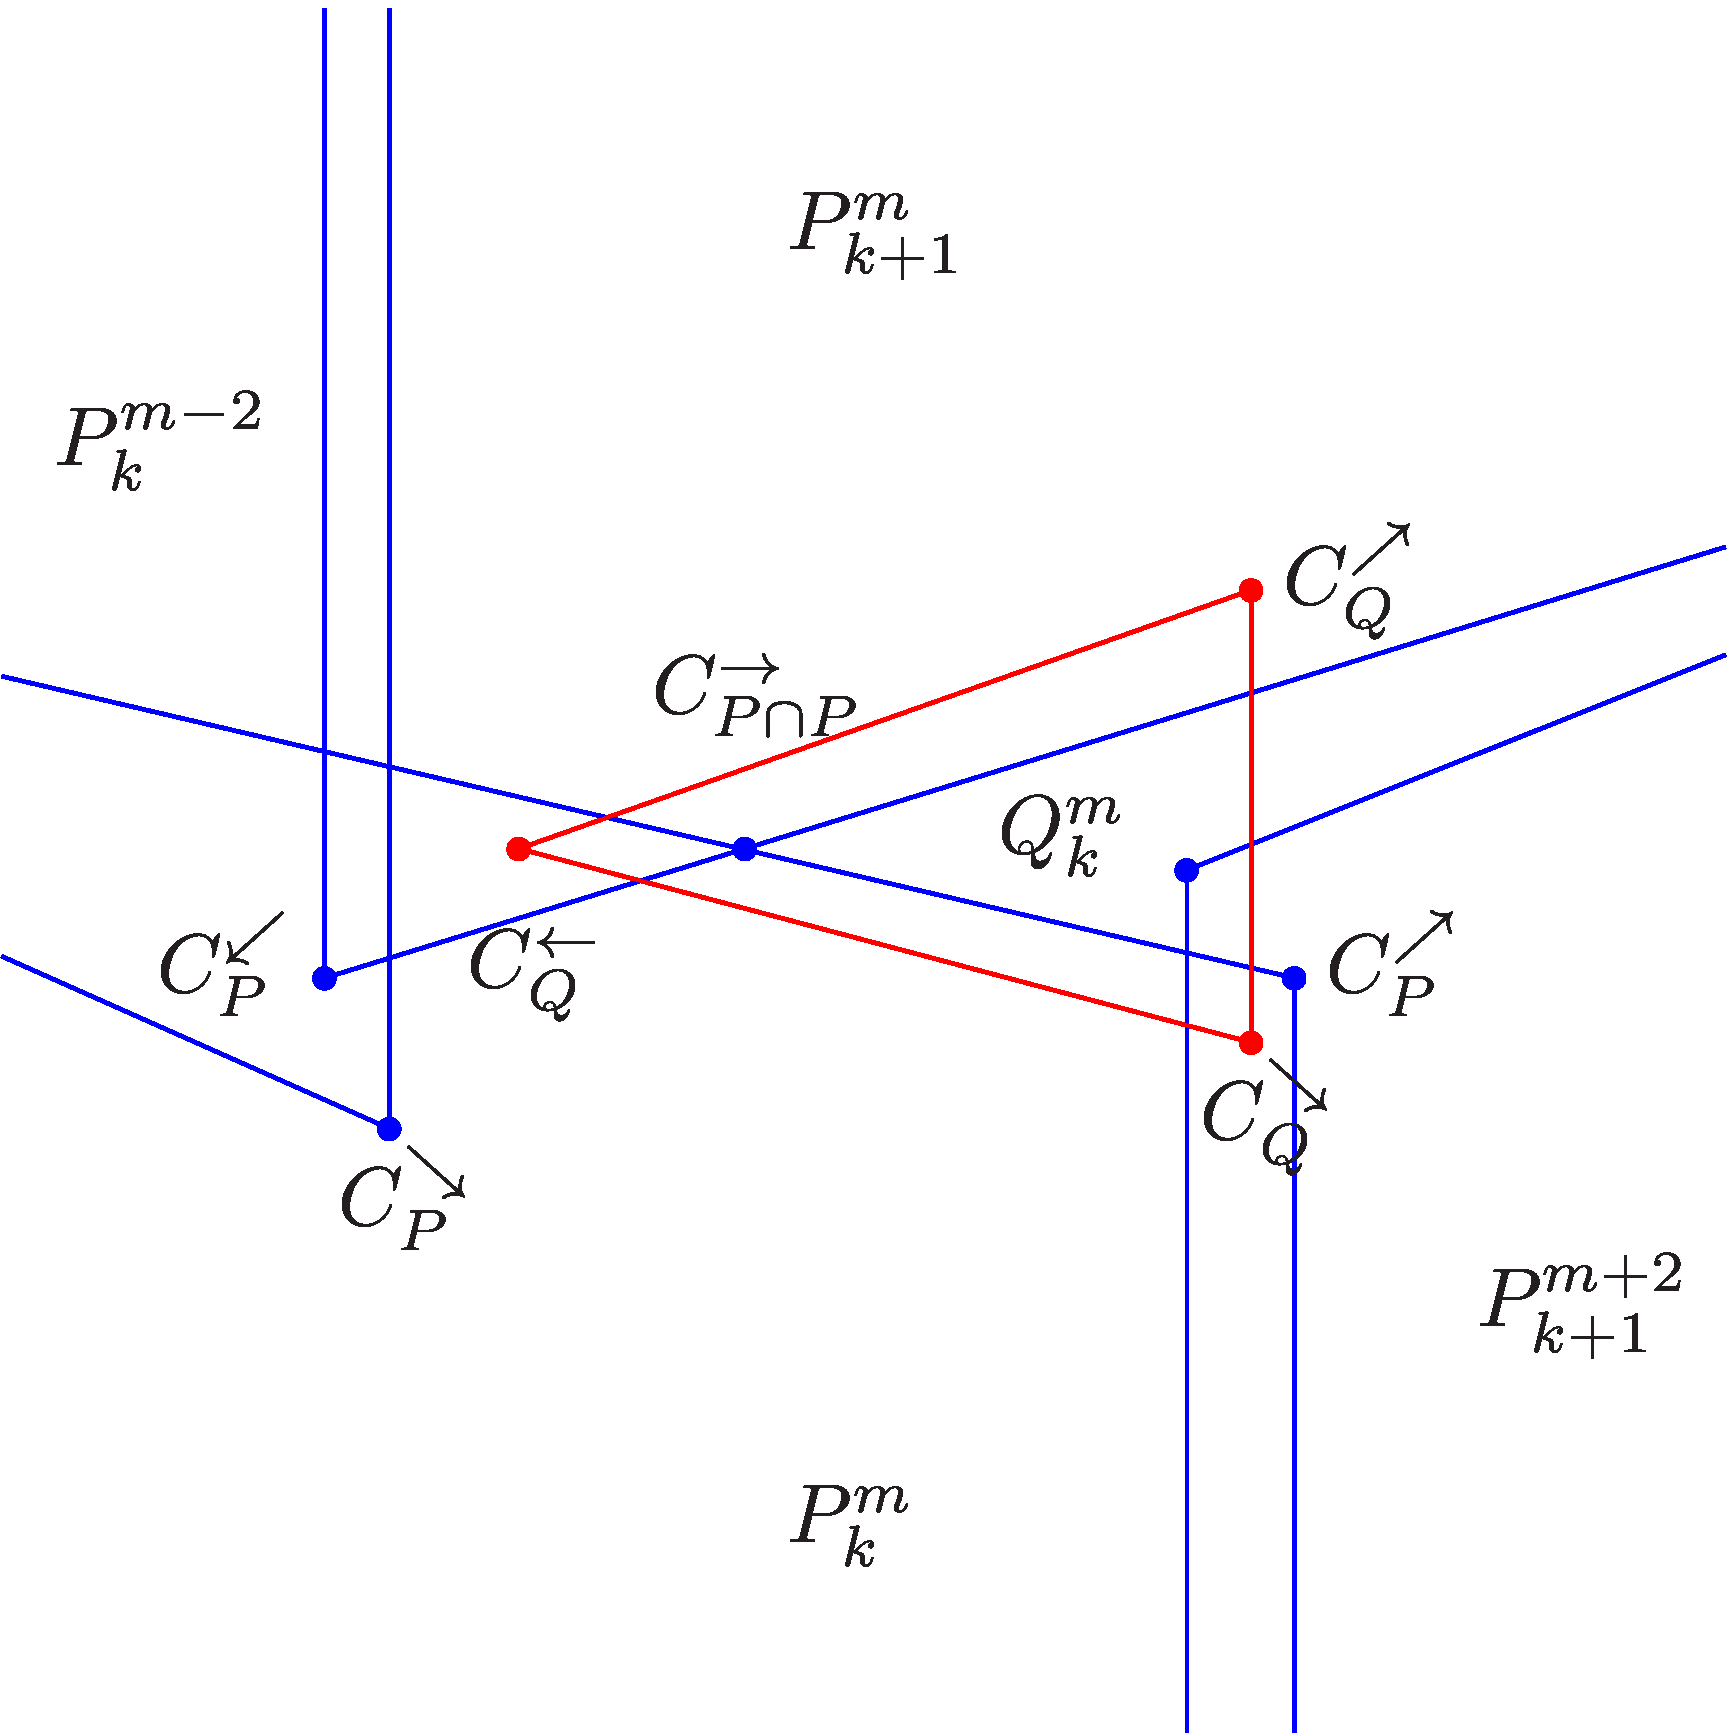
\includegraphics[width=.4 \textwidth]{../Figures/7/7.9c/result.png}
		\label{fig:add.change.schema.c}
	}
	\subfloat[]{
		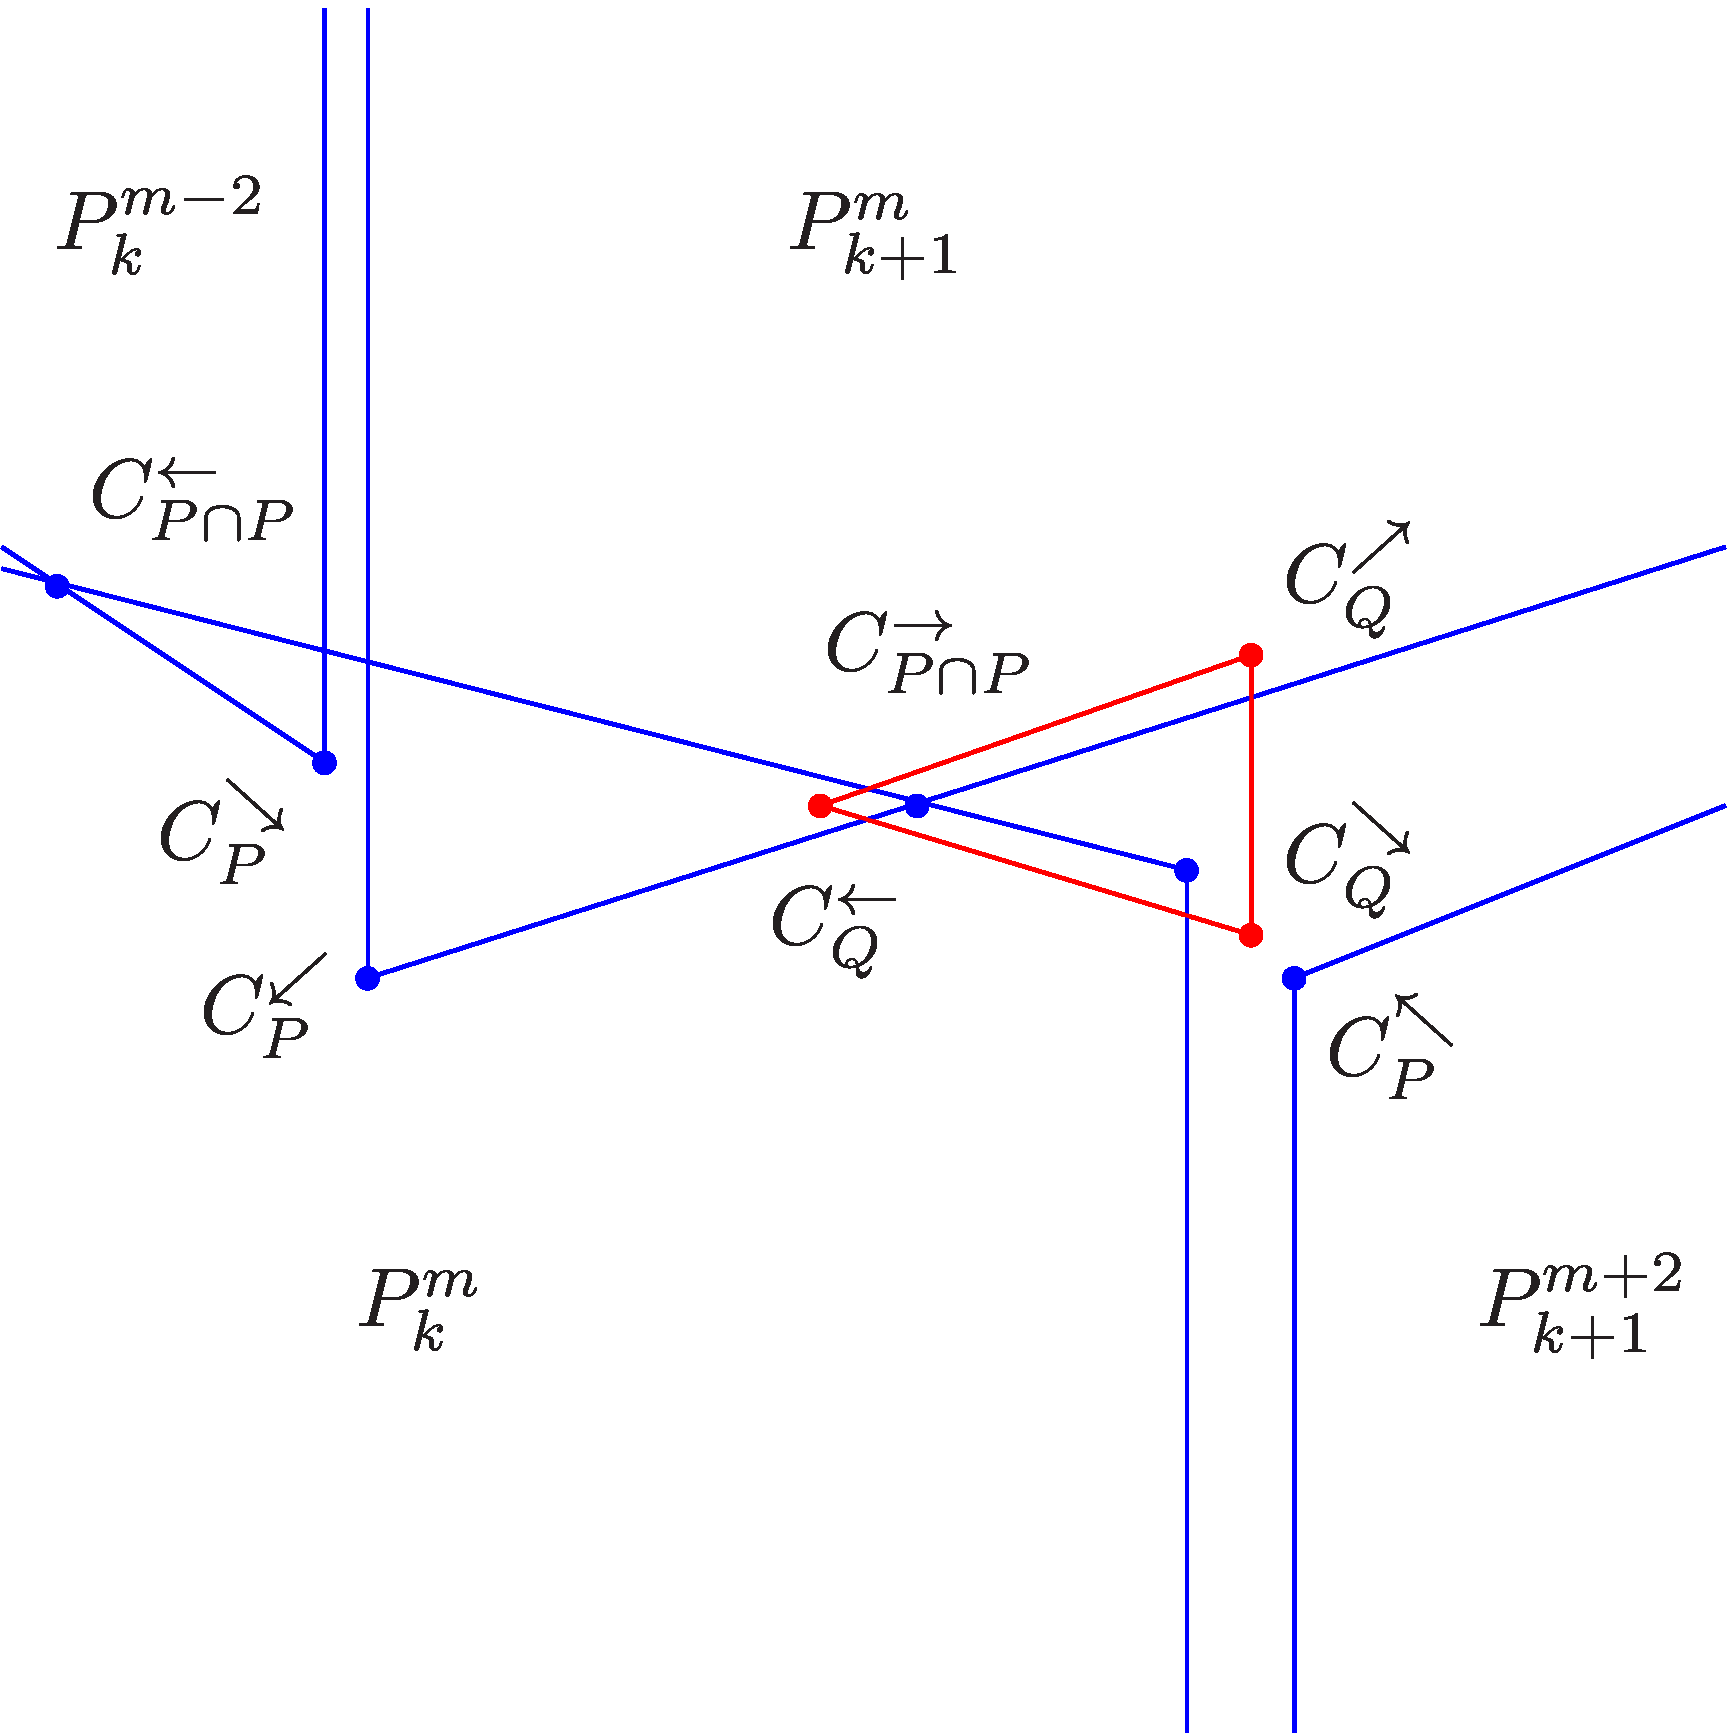
\includegraphics[width=.4 \textwidth]{../Figures/7/7.9d/result.png}
		\label{fig:add.change.schema.d}
	} \\
	\subfloat[]{
		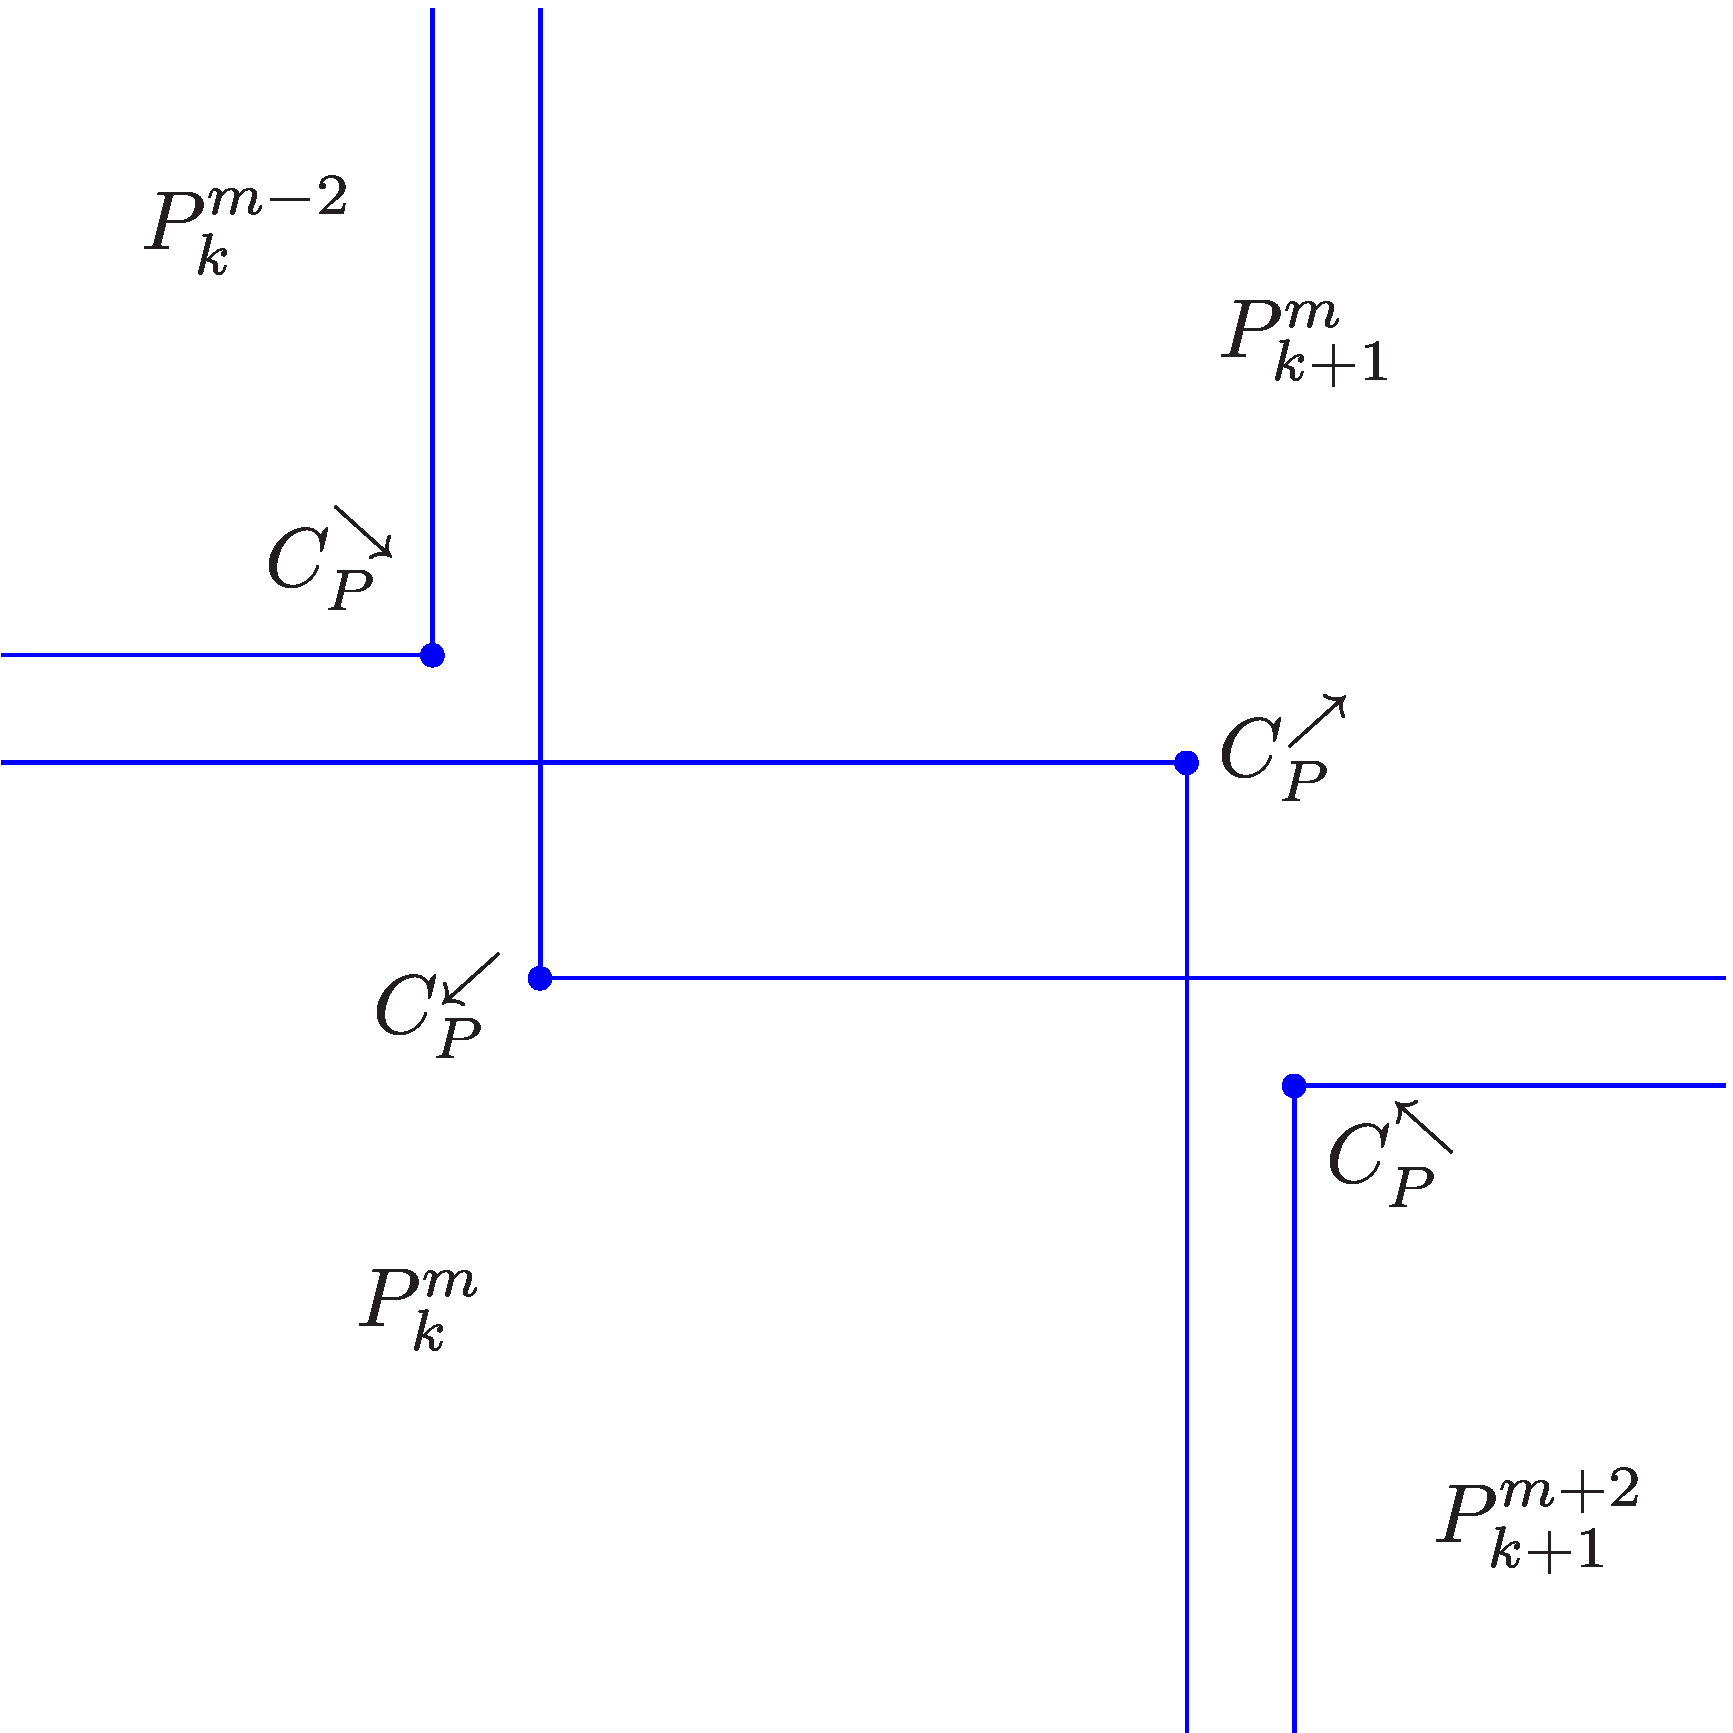
\includegraphics[width=.4 \textwidth]{../Figures/7/7.9e/result.png}
		\label{fig:add.change.schema.e}
	}
	\caption[Schematics of the boundaries of parameter regions associated with different symbolic sequences during the transition of the archetypal model to increasing branches]{
		Schematics of the boundaries of parameter regions associated with different symbolic sequences during the transition of the archetypal model to increasing branches.
		The boundaries of ``type A'' parameter regions are shown in blue while the boundaries of ``type B'' parameter regions are shown in red.
		Significant points where boundaries meet or cross are marked with dots.
	}
	\label{fig:add.change.schema}
\end{figure}

\Cref{fig:add.change.schema} shows multiple schematics that are used in this section to summarize all changes.
All schematics show some boundaries of the ``type A'' parameter regions $P^m_k, P^{m-2}_{k-1}, P^m_{k+1},$ and $P^{m+2}_{k+1}$ and all boundaries of the ``type B'' parameter region $Q^m_k$.
The ``type B'' parameter region is in-between all the ``type A'' parameter regions in the beginning.
This is shown in \Cref{fig:add.change.schema.a}.
The corners of the parameter regions are marked as follows.
The upper right corner of the ``type B'' parameter region in the middle is marked with the point $C_Q^\nearrow$.
Similarly, the lower right corner is marked with the point $C_Q^\searrow$ and the remaining corners with the points $C_Q^\nwarrow$ and $C_Q^\nwarrow$.
The corners of the ``type A'' parameter regions are marked analogously with $C_P^\nearrow, C_P^\searrow, C_P^\nwarrow,$ and $C_P^\swarrow$.
But here, the corners belong to different parameter regions.

The changes are summarized in the order they happen to the parameter regions that are considered in the previous sections.
This order might differ for different parameter regions.

First, the upper left corner $C_Q^\nwarrow$ of the lower right ``type A'' parameter region $P^{m+2}_{k+1}$ moves down and crosses the lower boundary of the upper right ``type A'' parameter region $P^m_{k+1}$.
This is visible in \Cref{fig:add.change.schema.b}.
The point where the two boundaries of the horizontally neighboring ``type A'' parameter regions cross is marked as $C_{P \cap P}^\leftarrow$ because this point is now the only left corner point of the overlapping parameter region $P^{m+2}_{k+1} \cap P^{m}_{k+1}$.
For higher values of $b_L$, the point $C_Q^\nwarrow$ moves further down which causes the point where the boundaries cross to move right.
In \Cref{fig:add.change.schema.c}, this crossing point is not visible anymore, since it moved out of the domain of the picture.
In \Cref{fig:add.change.schema.d}, it is visible again, but on the left side of the schema.
Strictly speaking, this is not the same point but the left boundary of the overlapping parameter region $P^m_k \cap P^{m-2}_{k}$.
This point then collides with the corner point $C_P^\nearrow$ which then causes the two ``type A'' parameter regions to not overlap anymore.
This final scenario can be seen in \Cref{fig:add.change.schema.e}.
In the spaces that opened up between the vertically neighboring ``type A'' parameter regions, there are big hybrid parameter regions $\left[P^{m+2}_{k+1} \mid P^{m}_{k+1}\right]$ and $\left[P^m_k \mid P^{m-2}_k\right]$, respectively.
The hybrid parameter regions are not shown in the schematics but while the overlapping parameter regions have only three boundaries, they too only have three boundaries and are bounded to the right only by one codimension-2 point.
At this point, their upper and lower boundaries meet.

As we can see in the schematics, this change starts first and finishes last.
While the described process occurs, another change starts happening.
The points $C_P^\searrow$ and $C_Q^\nearrow$ move down while the points $C_Q\searrow$ and $C_P^\nearrow$ move up.
As soon as the point $C_P^\swarrow$ crosses the upper boundary of $P^m_k$, the ``type A'' parameter regions $P^m_k$ and $P^m_{k+1}$ start to overlap.
This overlapping region is bounded to the right only by the point where the horizontal boundaries of those two parameter regions cross.
This point is marked as $C_{P \cap P}^\rightarrow$ in \Cref{fig:add.change.schema.c}.
Also at some parameter values the corner points $C_Q^\nwarrow$ and $C_Q^\searrow$ of the ``type B'' parameter region $Q^m_k$ in the middle collide.
This creates a codimension-2 point that bounds the parameter region $Q^m_k$ to the left, hence it is marked as $C_Q^\leftarrow$.
Both these newly created corner points move right, as can be seen in \Cref{fig:add.change.schema.d}.
Finally, the corner point $C_{P \cap P}^\rightarrow$ collides with the corner point $C_P^\nearrow$ and the two horizontal boundaries of the ``type A'' parameter regions stop crossing.
The overlapping parameter region $P^m_k \cap P^m_{k+1}$ is now bounded by four boundaries, as can be seen in \Cref{fig:add.change.schema.e}.
And the corner point $C_Q^\leftarrow$ crosses the right boundary of the ``type B'' parameter region, destroying the ``type B'' parameter region.

While that change is happening, one more change takes place.
This change does not happen by two boundaries crossing at one point like the last two changes.
Instead, the numeric evidence suggests that it happens at once.
The corner point $C_P^\nwarrow$ crosses the right boundary of $P^m_k$ at the same time, the lower right corner point of $P^{m}_{k}$ which is not pictured here crosses the left boundary of $P^{m+2}_{k+1}$.
This lower corner point is not pictured, but the lower right corner point of $P^{m-2}_k$ is pictured and marked as $C_P^\searrow$.
Here, the equivalent happens for the horizontally neighboring ``type A'' parameter regions $P^{m-2}_k$ and $P^m_{k+1}$.
In \Cref{fig:add.change.schema.c}, the horizontally neighboring ``type A'' parameter regions overlap and in \Cref{fig:add.change.schema.d}, the parameter regions do not overlap.
Instead, there is now space in-between the horizontally neighboring ``type A'' parameter regions.
In this space there now is a big hybrid parameter region and \gls{pal} structures, similar to the vertically neighboring ``type A'' parameter regions.

\subsubsection{Observations}

The local minima on branches $f_\A$ and $f_\C$ seem to be important for the ``type B'' parameter regions.
That means, parameter regions with coexisting asymmetrical cycles with the \textbf{same} period.
At the same time, these minima seem to prevent period-adding structures.
It will be proven next that ``type B'' parameter regions are impossible with only increasing branches.

\begin{lemma}[Number and Positions of Points of two Cycles on an Increasing Branch]
	Let $f_\X$ be an increasing branch of some model function $f$.
	If two cycles $\sigma_1$ and $\sigma_b$ have points on this branch, there are two possibilities for the relative number of points and relative position of the points.
	\begin{enumerate}
		\item Both cycles have the same number of points on the branch $f_\X$.
		      Let the first point of $\sigma_1$ be to the left of the first point of $\sigma_2$ on this branch w.l.o.g.
		      Then the last point of $\sigma_1$ is also to the left of the last point of $\sigma_2$ on this branch.
		      \Cref{fig:add.change.increasing.a} illustrates this case.
		\item One cycle has one more point on the branch $f_\X$.
		      Let $\sigma_1$ be the cycle with more points on this branch w.l.o.g.
		      Then the first point of $\sigma_1$ is to the left of the first point of $\sigma_2$ on this branch and the last point of $\sigma_1$ is to the right of the last point of $\sigma_2$ on this branch.
		      \Cref{fig:add.change.increasing.b} illustrates this case.
	\end{enumerate}
	\label{lemma:add.num.pos.points.increasing}
\end{lemma}

\begin{figure}
	\centering
	\subfloat[Same number of points]{
		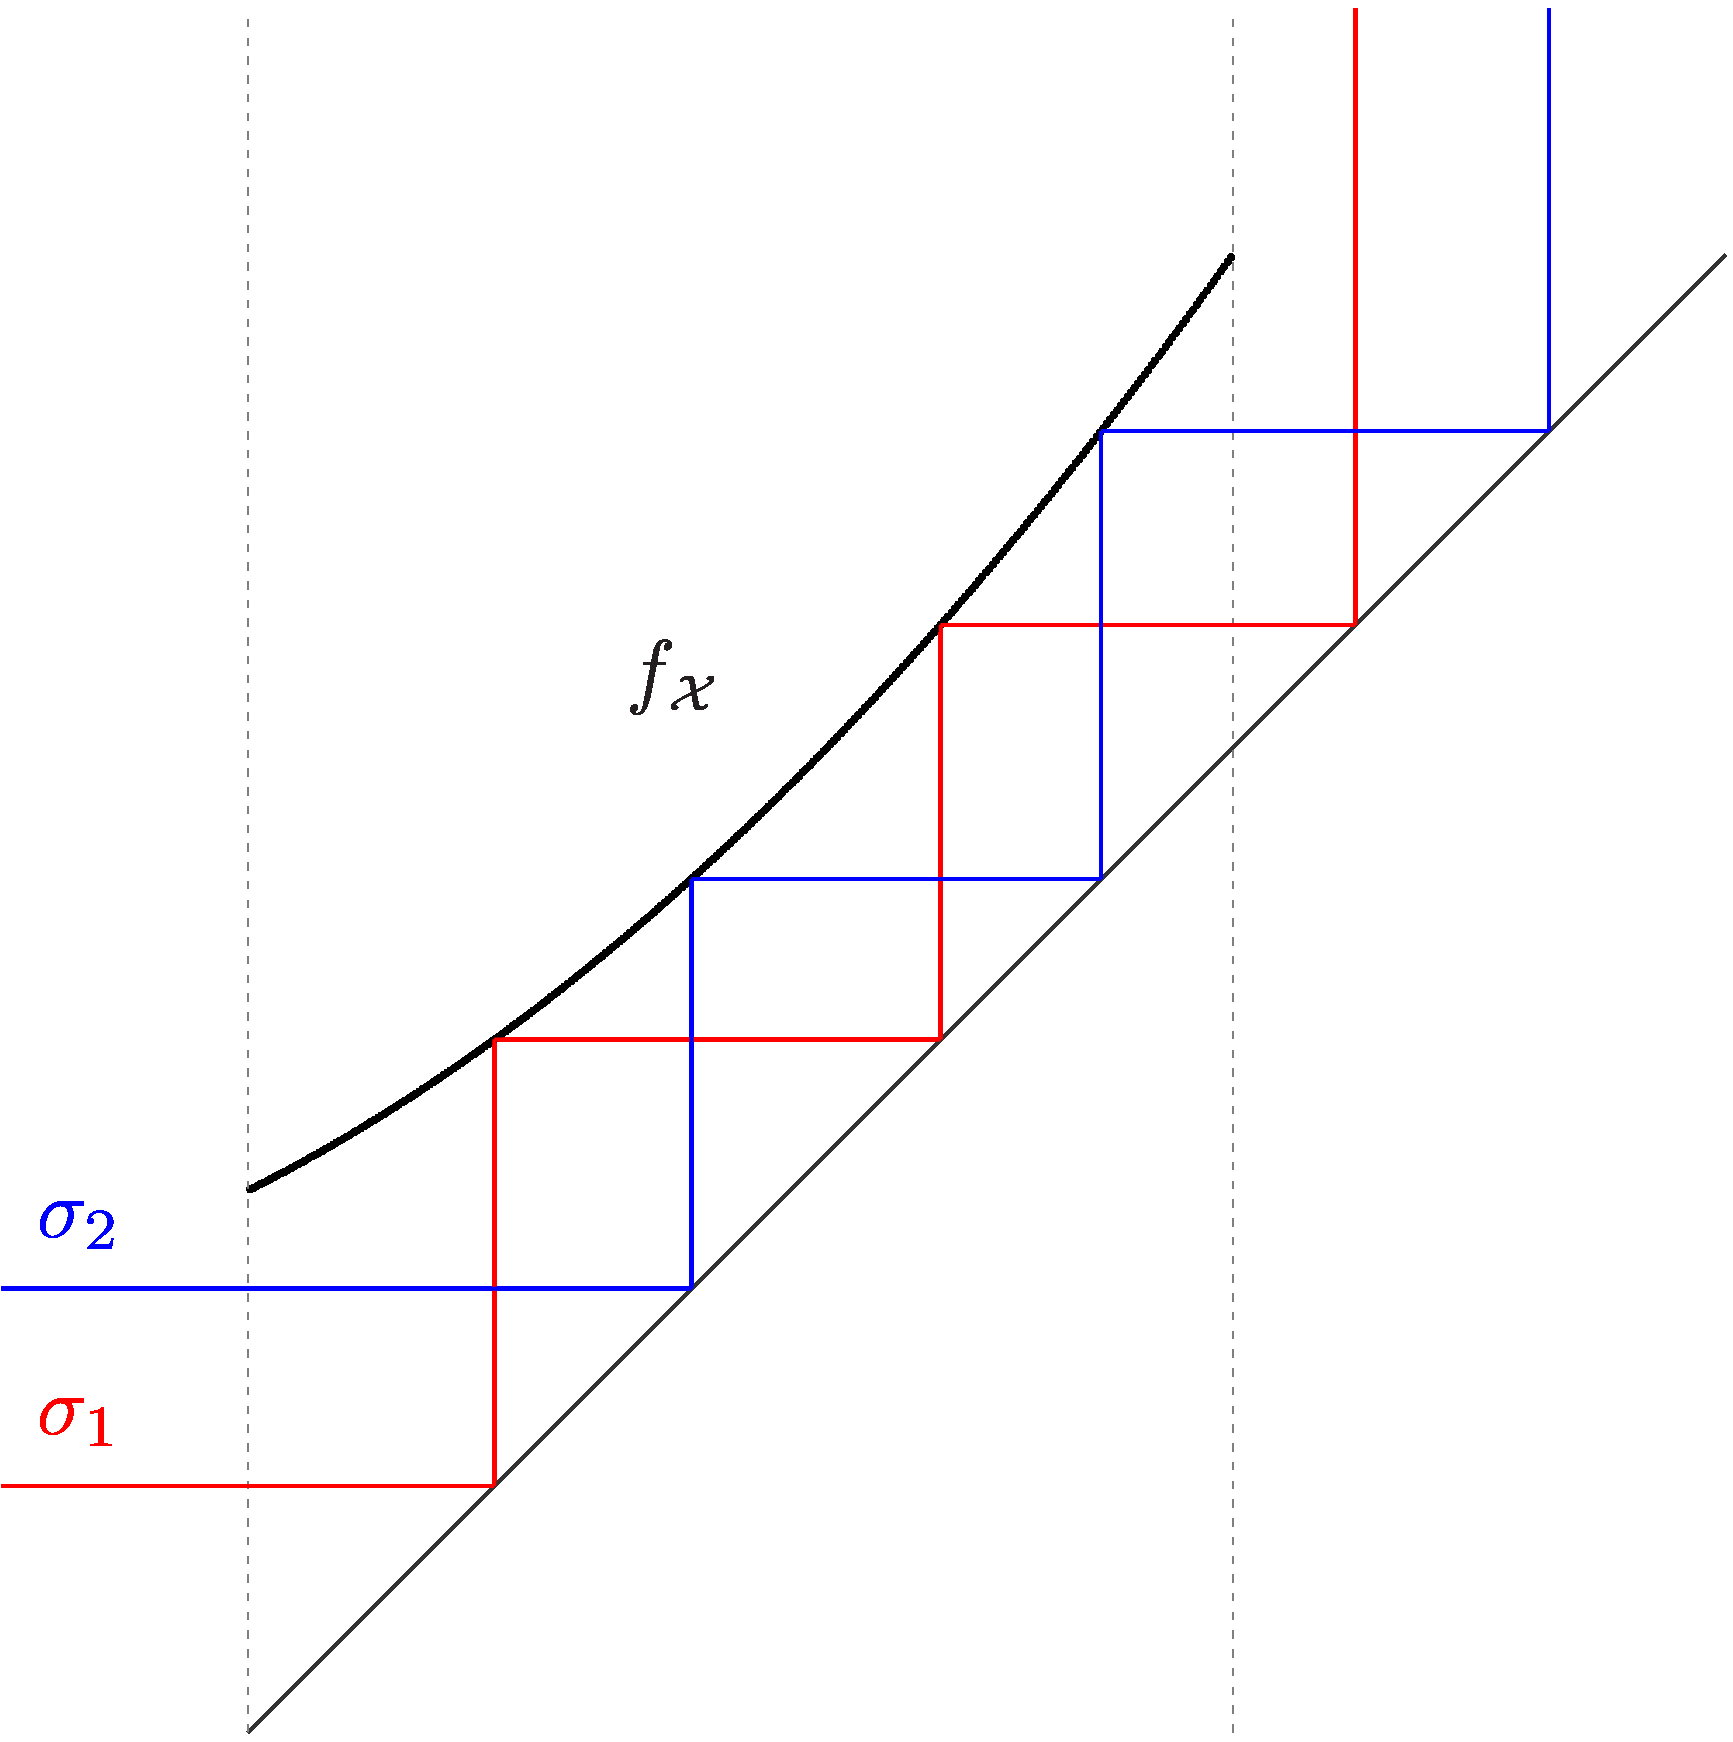
\includegraphics[width=.35 \textwidth]{../Figures/7/7.10a/result.png}
		\label{fig:add.change.increasing.a}
	} \quad
	\subfloat[Number of points differing by one]{
		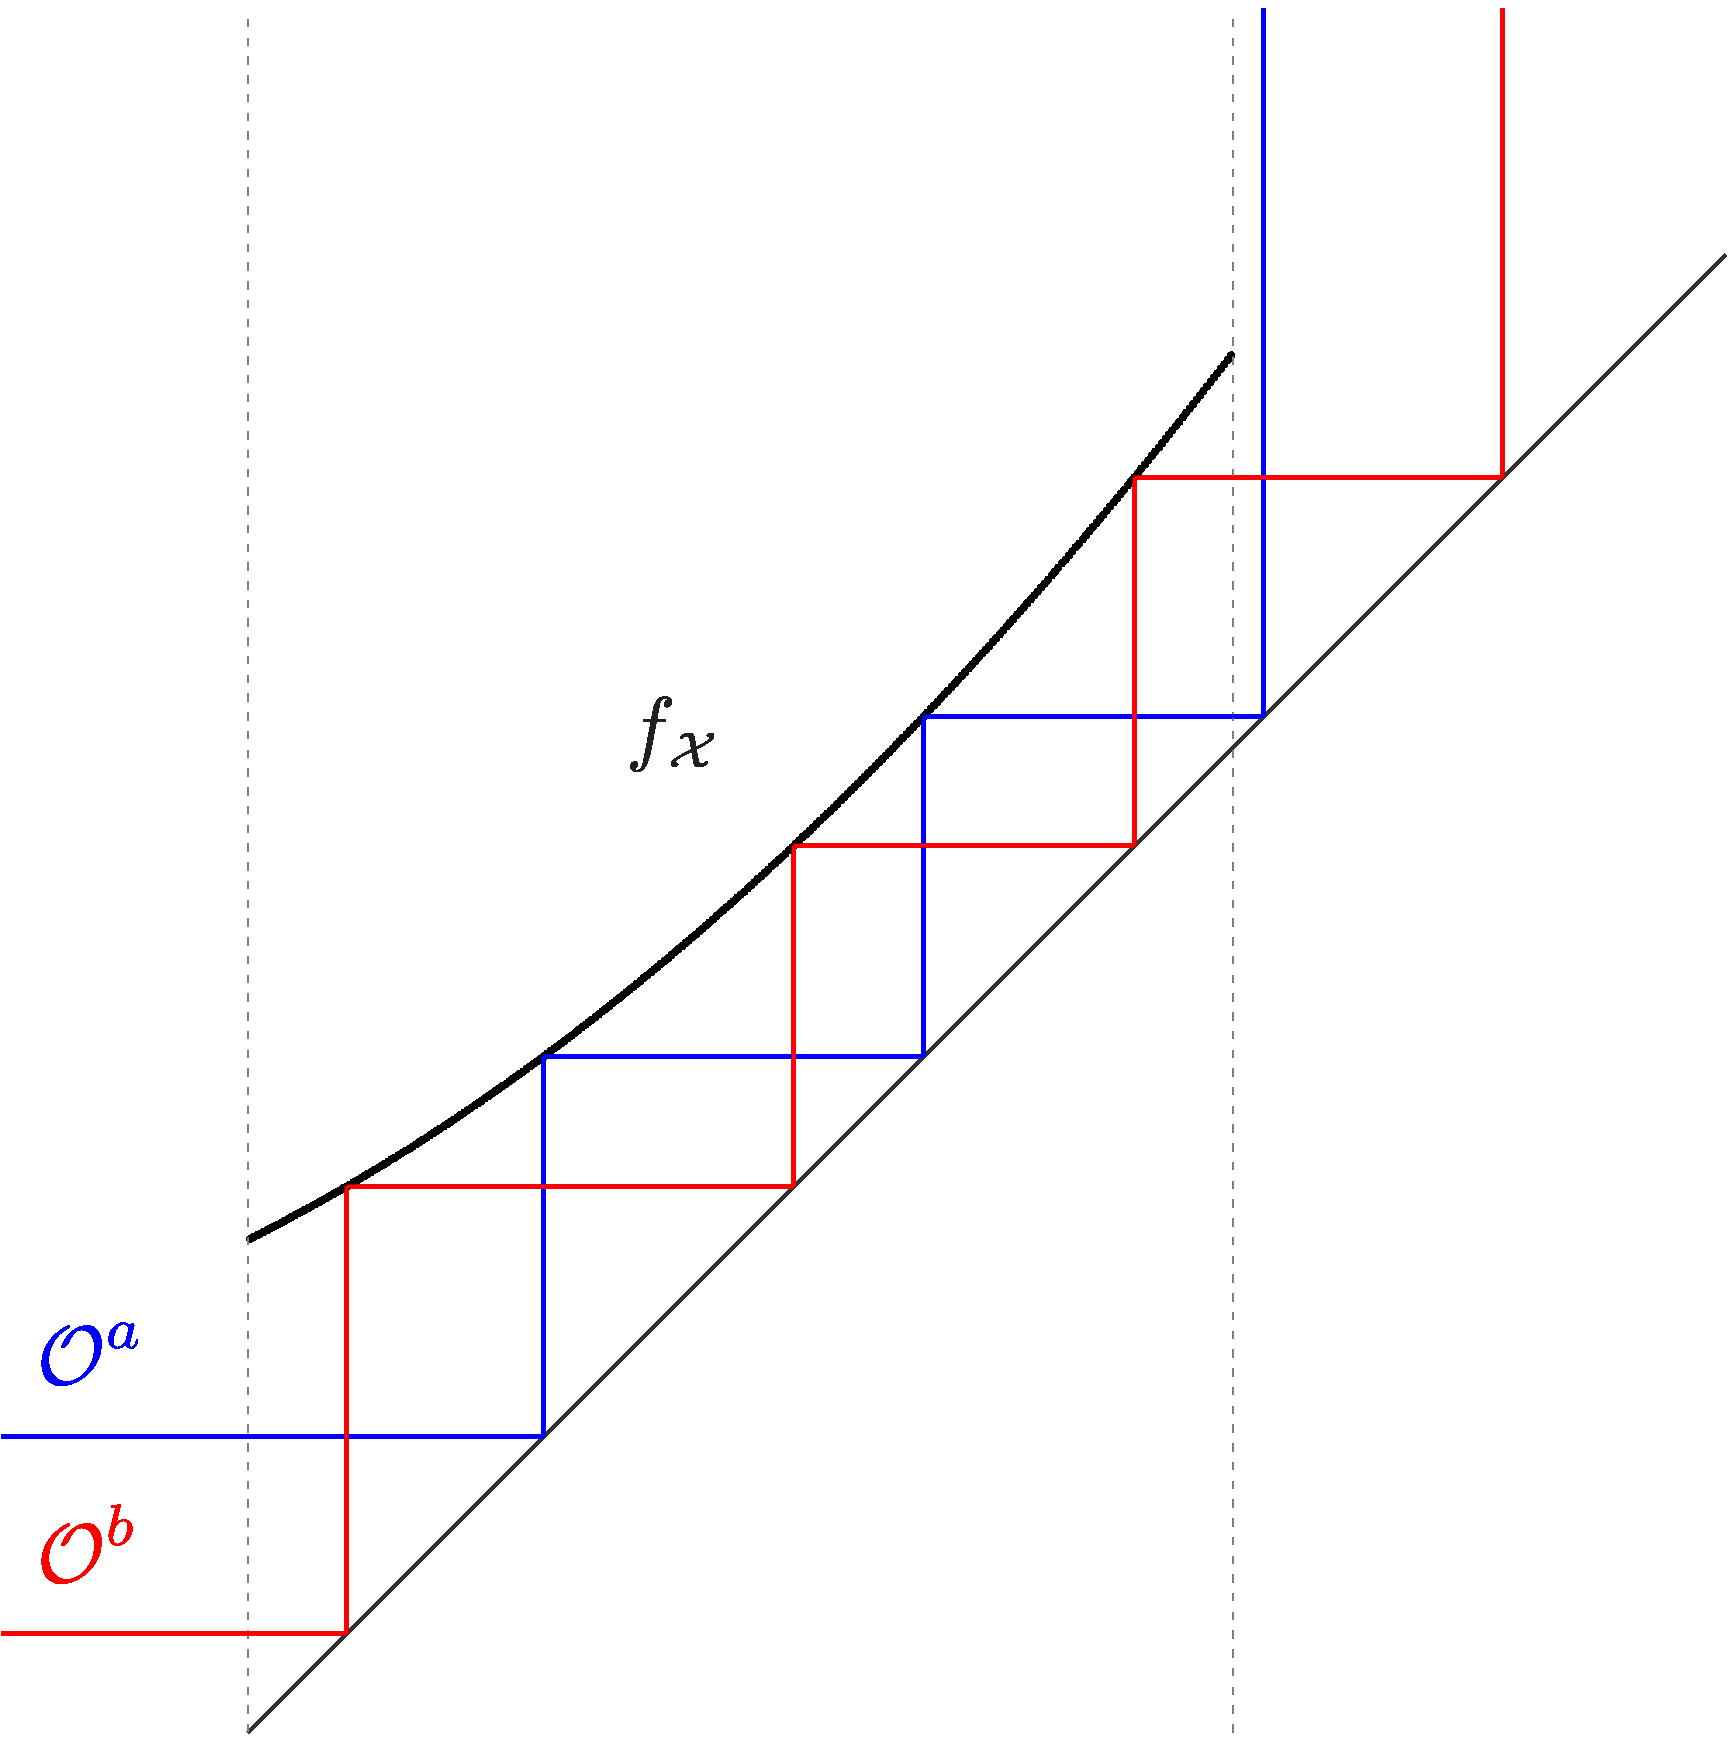
\includegraphics[width=.35 \textwidth]{../Figures/7/7.10b/result.png}
		\label{fig:add.change.increasing.b}
	}
	\caption[Illustration of the relative number and positions of the points of two cycles on an increasing branch]{
		Illustration of the relative number and positions of the points of two cycles on an increasing branch.
		Both figures show a function branch $f_\X$ and parts of two cycles, $\sigma_1$ shown in red and $\sigma_2$ shown in blue.
		(a) shows the case where both cycles have the same number of points on the branch $f_\X$ and the first point of $\sigma_1$ is to the left of the first point of $\sigma_2$ on this branch.
		(a) shows the case where the cycle $\sigma_1$ has one point more on the branch $f_\X$ than $\sigma_2$ and the first point of $\sigma_1$ is to the left of the first point of $\sigma_2$ on this branch.
	}
	\label{fig:add.change.increasing}
\end{figure}

\begin{theorem}[No ``Type B'' Parameter Regions with only Increasing Branches]
	The ``type B'' parameter regions are not possible in the increasing archetypal model.
	The minima on the branches $f_\A$ and $f_\C$ are essential for the bifurcation structure.
\end{theorem}

\begin{proof} \phantom{x} \\
	Let's assume that all branches of the archetypal model $f_\A, f_\B, f_\C,$ and $f_\D$ are increasing.
	And let $\sigma_1$ and $\sigma_2$ be ``type B'' twin cycles.
	The following conditions are true for such cycles.
	\begin{subequations}
		\begin{align}
			|\sigma_1|_\A - 1 & = |\sigma_2|_\A \label{equ:add.change.conseq.sigmaA} \\
			|\sigma_1|_\B + 1 & = |\sigma_2|_\B \label{equ:add.change.conseq.sigmaB} \\
			|\sigma_1|_\C + 1 & = |\sigma_2|_\C \label{equ:add.change.conseq.sigmaC} \\
			|\sigma_1|_\D - 1 & = |\sigma_2|_\D \label{equ:add.change.conseq.sigmaD}
		\end{align}
	\end{subequations}

	For \Cref{equ:add.change.conseq.sigmaA} to hold, the first point of  $\sigma_1$ needs to be to the left of first point of  $\sigma_2$ on the branch $f_\A$, because  $\sigma_1$ has one point more on this branch than  $\sigma_2$ and this branch is increasing.
	At the same time, the last point of  $\sigma_1$ must be to the right of the last point of  $\sigma_2$ on this branch.

	The order of the first points on the next branch, $f_\B$, is the same as for the last points on the branch $f_\A$.
	So the first point of  $\sigma_2$ is to the left of the first point of  $\sigma_1$ on this branch.
	For \Cref{equ:add.change.conseq.sigmaB} to hold, the last point of  $\sigma_2$ must be to the right of the last point of  $\sigma_1$ on this branch per the same logic as before.

	The order of the first points on the next branch, $f_\C$, is the same as for the last points on the branch $f_\B$.
	So the first point of  $\sigma_1$ is to the left of the first point of  $\sigma_2$ on this branch.
	This is a contradiction, since the first point of  $\sigma_1$ on the branch $f_\A$ is also to the left of the first point of  $\sigma_2$ on that branch.
	This violates the symmetry.
	Also, \Cref{equ:add.change.conseq.sigmaC} cannot be fulfilled if the first point of  $\sigma_1$ is to the left of the first point of  $\sigma_2$ on the branch $f_\C$, since the first point of  with more points, $\sigma_2$ in this case, on the branch must be to the left of the first point of the other cycle on that branch if the branch is increasing.

	\hfill $\blacksquare$
\end{proof}

